\fullsys (\sys) is the abstraction of a group of batteryless intermittent sensors. \sys orchestrates its nodes power cycles using a distributed approach (instead of relying on a master powerful node to coordinate coalesced nodes activities). 
%\sys seeks maximum time span of its underlying coalesced nodes through a distributed approach instead of a master node that orchestrates coalesced nodes on/off cycles. 

\subsection{Intermittent Nodes' Power Cycles Distribution}
To ensure an efficient distribution of the intermittent nodes' uptimes, an explicit or implicit control methods can be applied: (i) explicit control of nodes' power cycles requires inter-nodes communication. Communication between batteryless nodes requires ultra low power communication regimes to be efficient. Recent advancements in passive visible light communication~\cite{Marco} and ambient radio frequency backscattering~\cite{} demonstrate the feasibility of extremely energy efficient communication between batteryless nodes. Once messages exchange is possible, an intermittent node duty is to estimate the number of active nodes in its time slot and to decide on leaving this power cycle of maintaining it (Figure~\ref{xxx}). Nodes can influence their power cycles by altering their load---low power consumption extends a node's uptime and delays its off-time, and high power consumption has an inverse effect. (ii) implicit control of nodes' power cycles approach seeks to use a random process to "ideally" uniformly distribute nodes' on/off cycles over the \sys's power cycle: when all the nodes complete their individual power cycles. \sys takes advantage of the randomized nature of the ambient energy to distribute its coalesced nodes. 

In this paper we opt to explore the implicit nodes distribution control approach as it is simpler and requires less overhead than explicit control methods~\footnote{The hardware used to demonstrate the feasibility of passive light communication and ambient RF backscattering are not open source and re-making it is beyond the scope of this study \todo{add the references to Marco's paper and ambient RF paper}}.


\paragraph{Implicit Control: Exploiting Solar Power}
%
The implicit control methods have the advantage of not requiring control messages exchanging and processing. 
%
\begin{figure}
	\centering
		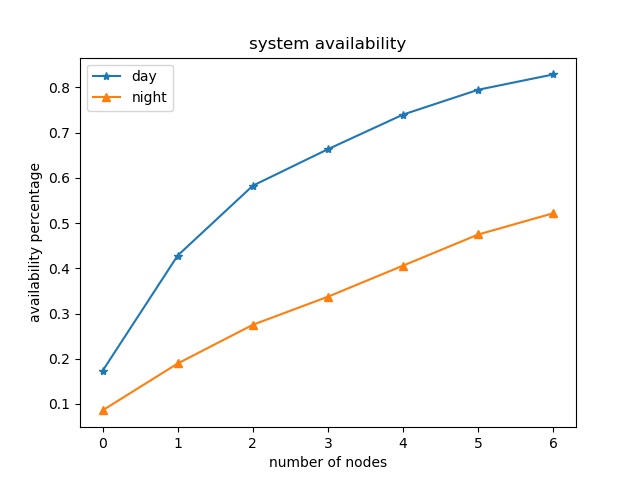
\includegraphics[width=\columnwidth]{figures/solarPoweredCoIS.png}
	\caption{Implicit \fullsys' nodes distribution using solar power harvesting randomization}
	\label{fig:solarPwrCoIS}
\end{figure} 

Figure~\ref{fig:solarPwrCoIS} shows an implicit solar power based \sys's nodes distribution when they are powered by artificial light (during night) and sunlight (during day). 





\subsection{Sensing on Intermittent Power}
